
\documentclass[12pt]{article}

% Layout.
\usepackage[top=1in, bottom=0.75in, left=1in, right=1in, headheight=1in, headsep=6pt]{geometry}

% Fonts.
\usepackage{mathptmx}
\usepackage[scaled=0.86]{helvet}
\renewcommand{\emph}[1]{\textsf{\textbf{#1}}}

% TiKZ.
\usepackage{tikz, pgfplots}
\usetikzlibrary{calc,trees,positioning,arrows,fit,shapes,calc}
\pgfplotsset{compat = newest}
\tikzset{
  jumpdot/.style={mark=*,solid},
  excl/.append style={jumpdot,fill=white},
  incl/.append style={jumpdot,fill=black},
}
 
\pgfplotsset{my style/.append style={axis x line=middle, axis y line=
middle, xlabel={$x$}, ylabel={$y$}, axis equal }}

% Misc packages.
\usepackage{amsmath,amssymb,latexsym}
\usepackage{graphicx}
\usepackage{array}
\usepackage{xcolor}
\usepackage{multicol}

% Commands to set various header/footer components.
\makeatletter
\def\doctitle#1{\gdef\@doctitle{#1}}
\doctitle{Use {\tt\textbackslash doctitle\{MY LABEL\}}.}
\def\docdate#1{\gdef\@docdate{#1}}
\docdate{Use {\tt\textbackslash docdate\{MY DATE\}}.}
\def\doccourse#1{\gdef\@doccourse{#1}}
\let\@doccourse\@empty
\def\docscoring#1{\gdef\@docscoring{#1}}
\let\@docscoring\@empty
\def\docversion#1{\gdef\@docversion{#1}}
\let\@docversion\@empty
\makeatother

% Headers and footers layout.
\makeatletter
\usepackage{fancyhdr}
\pagestyle{fancy}
\fancyhf{} % Clears all headers/footers.
\lhead{\baselineskip 30pt
%\emph{\@doctitle\hfill\@docdate}
\emph{\@docdate\hfill\@doctitle}
\ifnum \value{page} > 1\relax\else\\
\emph{Name: \rule{3.5in}{1pt}\hfill \@docscoring}\fi}
\rfoot{\emph{\@docversion}}
\lfoot{\emph{\@doccourse}}
\cfoot{\emph{\thepage}}
\renewcommand{\headrulewidth}{0pt}%
\makeatother

% Paragraph spacing
\parindent 0pt
\parskip 6pt plus 1pt

% A problem is a section-like command. Use \problem{5} to
% start a problem worth 5 points.
\newcounter{probcount}
\newcounter{subprobcount}
\setcounter{probcount}{0}
\newcommand{\problem}[1]{%
\par
\addvspace{4pt}%
\setcounter{subprobcount}{0}%
\stepcounter{probcount}%
%\makebox[0pt][r]{\emph{\arabic{probcount}.}\hskip1ex}\emph{[#1 points]}\hskip1ex}
\makebox[0pt][r]{\emph{\arabic{probcount}.}\hskip1ex}\emph{[#1 \ifnum1=0#1\relax point\else points\fi]}\hskip1ex}
%\textbf{(#1 \ifnum1=0#1\relax thing\else things\fi
\newcommand{\thesubproblem}{\emph{\alph{subprobcount}.}}

% Subproblems are an enumerate-like environment with a consistent
% numbering scheme. 
% Use \begin{subproblems}\item...\item...\end{subproblems}
\newenvironment{subproblems}{%
\begin{enumerate}%
\setcounter{enumi}{\value{subprobcount}}%
\renewcommand{\theenumi}{\emph{\alph{enumi}}}}%
{\setcounter{subprobcount}{\value{enumi}}\end{enumerate}}

% Blanks for answers in normal and math mode.
\newcommand{\blank}[1]{\rule{#1}{0.75pt}}
\newcommand{\mblank}[1]{\underline{\hspace{#1}}}
\def\emptybox(#1,#2){\framebox{\parbox[c][#2]{#1}{\rule{0pt}{0pt}}}}

% Misc.
\renewcommand{\d}{\displaystyle}
\newcommand{\ds}{\displaystyle}
\def\bc{\begin{center}}
\def\ec{\end{center}}
\def\be{\begin{enumerate}}
\def\ee{\end{enumerate}}

\newcommand{\ans}{\rule{2 in}{.5pt}}
\newcommand{\bigans}[1]{\rule{#1 in}{.5pt}}

\doctitle{Math F251X: Quiz 2}
\docdate{Fall 2026}
\doccourse{UAF Calculus I}
\docversion{v-1}
\docscoring{\blank{0.8in} / 25}
\begin{document}
\textbf{Please circle your section:} \hfill 901 (Gossell)  \hfill 902 (Gossell) \hfill 903 (Graves-McCleary)\\

No aids (book, calculator, etc.) are permitted.  {\bf Show all work for full credit.}

%Problem
\problem{10} Consider the graph of $f(x)=\sqrt[3]{x-2}+1$ given below:

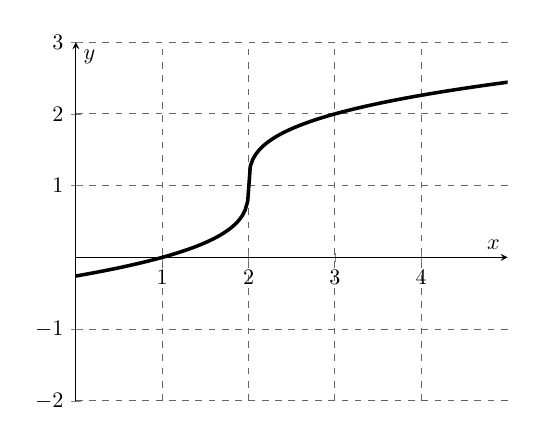
\begin{tikzpicture}[scale=0.8]
 \begin{axis}[
    xmin = 0, xmax = 5,
    ymin = -2, ymax = 3, xtick={0,1,...,4}, ytick={-2,...,3},
    grid=both, grid style={ thin, black!60, dashed},axis x line=middle, axis y line=
middle, xlabel={$x$}, ylabel={$y$}]
    \addplot[ultra thick, ->,samples=200,
        domain = 0:6,
    ] {sign(x-2)*abs(x-2)^(1/3)+1};
    %\addplot[thick,->] coordinates {(2,1) (3,2)};
\end{axis}
\end{tikzpicture}

\begin{subproblems}
\item Find the equation of the {\bf secant line} passing through the points $(2,1)$ and $(3,2)$. \\
  \vfill
  \vfill
  \vfill
  
\item Sketch the secant line from part (a) on the graph above. Label it ``Secant Line''.\\
  \vfill
  
\item The table below lists the slope ($m_{sec}$) of the secant line passing through the point $(3,2)$ and the point $(x, f(x))$ for several values of $x.$ \\

\begin{tabular}{l || c|c|c|c|c|c}
$x$ & 2.9 & 2.99 & 2.999 & 3.001 & 3.01 & 3.1 \\\hline
$f(x)$ & 1.96549 & 1.99666 & 1.99967 & 2.00033 & 2.00333 & 2.03228 \\\hline
$m_{sec}$ & 0.34511 & 0.33445 & 0.33344 & 0.33322 & 0.33278 & 0.32280 \\
\end{tabular}\\

Use the information in the table to {\bf estimate} the slope of the {\bf tangent line} to $f(x)$ at $(3,2)$.
  \vfill

\item Use the slope from part (c) to write the equation of the tangent line at $(3,2)$.
  \vfill
  \vfill
  \vfill
  
\item Sketch the tangent line from part (d) on the graph above. Label it ``Tangent Line''.\\
  \vfill
\end{subproblems}

\newpage


\problem{7} The height of a hot air balloon after $t$ minutes is given by $\displaystyle h(t)=1500 - \frac{3000}{1+2^t}$ feet.\\
\begin{subproblems}
\item Find the height of the hot air balloon at time $t=0$, $t=1$, and $t=2$.
\vfill
$h(0)=\mblank{.6in}$ \hspace{.5in} $h(1)=\mblank{.6in}$ \hspace{.5in} $h(2)=\mblank{.6in}$\\

\item Find the {\bf average velocity} of the hot air balloon during the first minute (from $t=0$ to $t=1$).
\vfill
\item Find the {\bf average velocity} of the hot air balloon during the next minute (from $t=1$ to $t=2$). Based on this, do you think the ballon is speeding up or slowing down?
\vfill
\end{subproblems}

\problem{8} Use the graph of the function $H(x)$ (drawn below) to answer the questions. Assume $H(x)$ has a vertical asymptote at $x=5.$ For each problem below, give the most complete answer; if the limit is infinite, indicate that with $+\infty$ or $-\infty$. If the limit does not exist, write DNE. \\

\begin{center}
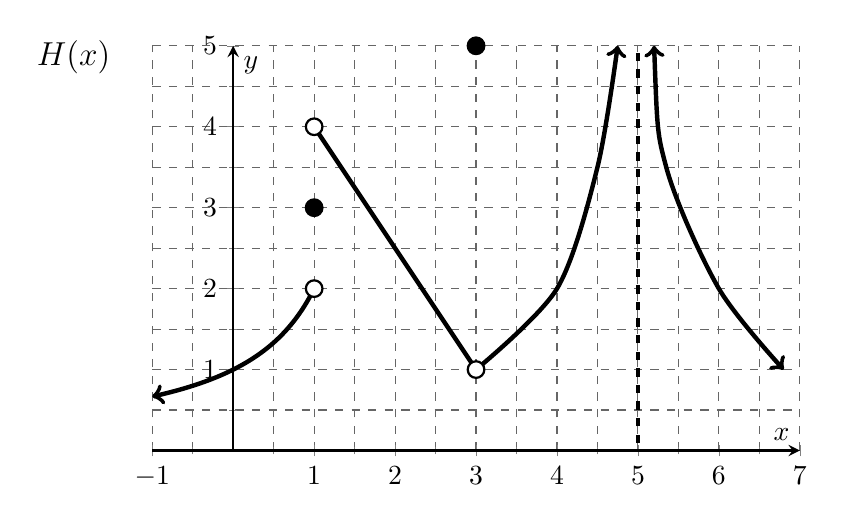
\begin{tikzpicture}
\begin{axis}[scale=1.2, thick, my style, xtick={-2,...,7}, ytick={-1, 0,...,5},
xmin=-1, xmax=7, ymin=0, ymax=5, minor y tick num=1,
        minor x tick num=1, mark size=3.0pt, grid=both, grid style={ thin, black!60, dashed}, axis equal image]
% %%asymptote
\addplot[dashed,<->, ultra thick] coordinates {(5,-2) (5,6)};       
%%points solid
\addplot[mark=*,only marks] coordinates {(1,3)(3,5)};
%%points open
\addplot[mark=*,fill=white,only marks] coordinates {(1,2)(1,4)(3,1)};
%%Curves
\addplot[<-,ultra thick, smooth, variable=\x, samples=100, domain=-1:1] plot(\x,{-2/(\x-2)});
%\addplot[ultra thick, smooth,<-] coordinates {(-3,4) (-2,3.5) (0,2)(1,0.5)};
\addplot[ultra thick, smooth] coordinates {(1,4) (3,1)};
\addplot[ultra thick, smooth,->] coordinates {(3,1) (4,2) (4.5,3.5)(4.75,5)};
%\addplot[ultra thick, smooth,->] coordinates {(2,2) (2.5,2.3) (2.7,4.5) (2.8,6)};
\addplot[ultra thick, smooth,<->] coordinates {(5.2,5) (5.35,3.5) (6,2)(6.8,1)};       
\end{axis}
\node at (-1,5){\large{$H(x)$}};
\end{tikzpicture}
\end{center}

\begin{subproblems}
\begin{multicols}{4}
\item $H(1)=\mblank{.5in}$
\item $\d{\lim_{x \to\; 1^-} H(x)=\mblank{.3in}}$
\item $\d{\lim_{x \to\; 1^+} H(x)=\mblank{.3in}}$
\item $\d{\lim_{x \to\; 1} H(x)=\mblank{.4in}}$
\end{multicols}
\vspace{0.1in}
\begin{multicols}{4}
\item $\d \lim_{x\to\; 2}H(x)=\mblank{.4in}$
\item $H(3)=\mblank{.5in}$
\item $\d \lim_{x\to\; 3}H(x)=\mblank{.4in}$
\item $\d{\lim_{x \to 5} H(x)=\mblank{.4in}}$
\end{multicols}
\end{subproblems}



\end{document}
%%% Local Variables:
%%% mode: LaTeX
%%% TeX-master: t
%%% End:
